%% ----------------------------------------------------------------
%% cyk.tex -- main
%% ----------------------------------------------------------------

\documentclass[10pt]{article}
\usepackage{amsmath}
\usepackage{amsfonts}
\usepackage{mathtools}
\usepackage[dvipsnames]{xcolor}
\usepackage{subcaption}
\usepackage{graphicx}
\usepackage{algorithm}
\usepackage[noend]{algpseudocode}
\floatname{algorithm}{Algorithm}
\usepackage{enumitem}
\usepackage{tikz}
\usepackage{forest}
\usetikzlibrary{shapes,positioning}
\usepackage{hyperref}
\usepackage[capitalise, noabbrev]{cleveref}
\newcommand{\todo}[1]{{\color{red}#1}}

% Bibliography stuff
\usepackage[
    backend=biber,  
    style=ieee,
    sorting=ynt
]{biblatex}
\addbibresource{main.bib}


%% ----------------------------------------------------------------

\title{Evaluation of the Cocke-Younger-Kasami Algorithm}
\author{Salome Müller}
\date{\today}

\begin{document}

%% Make the title
\maketitle

%% Write the abstract
\begin{abstract}
    The Cocke Younger Kasami algorithm can solve the membership problem for context free grammars in $O(n^3)$.
    For this report three different approaches to the algorithm are implemented and evaluated.
    The evaluation shows that the bottom-up approach is faster on average, while top-down has very fast running times in best-case.
    Further, bottom-up is specialized to operate on linear grammars, yielding running times in $O(n^2)$.
    The bottom-up approach can also be used to calculate the number of errors and correct the input string, such that the result belongs to the language of the grammar.
    While the correction of the string has linear running time and proceeds very fast, the generalized bottom-up algorithm is much slower than the original bottom-up algorithm.
\end{abstract}

\pagebreak
\tableofcontents
\pagebreak

%% Include all chapters
\section*{Introduction}
\todo{write the introduction}
% We implemented and tested three approaches for determining, whether a word is part of the language of a context free Grammar, namly a naive approach, the bottom-up CYK-algorithm, and a top down approach with memoization.
% We analysed the implementations and cam to some conclusions.
\section{Background}
\label{sec:backgrund}

The Cocke-Younger-Kasami algorithm, which we analyse in this report, solves the membership problem for context free grammars.
In this section we show what a context-free grammar is and how the algorithm operates on it.
Further, we introduce the three approaches for implementing the algorithm which were used in the evaluation.

\subsection{Context-Free Grammar}
\textbf{Context-free grammars} (CFG) are used to formalize different types of languages.
They can, for example, be used in computer science, to define the structure of programming languages or in linguistics to define the structure of any language.

A CFG contains a set of rules, also called productions.
Starting from a certain variable, this productions can be applied to get a sequence of terminal symbols, for example a sentence of the English language.
The sequences that can be generated with a CFG build a language, the grammars \textbf{context-free language} (CFL).

Formally, we define a CFG $G$ by the 4-tuple $G=(V,T,P,S)$.
$V$ and $T$ are two finite, disjoint sets containing all \textbf{variables} and \textbf{terminal} symbols respectively.
The variables are also called non-terminals.
$P$ is the set of \textbf{productions} and $S\in V$ is the \textbf{start symbol}.

The productions are of the form $A\rightarrow\alpha$, where $A$ is a variable in $V$ and $\alpha$ is a string of symbols from $(V\cup T)^*$.
If $P$ contains multiple productions for one non-terminal we abbreviate these productions as $A\rightarrow \alpha_1 | \alpha_2 | \dots |\alpha_k $, where $\alpha_i$, $i\in {1\dots k}$ is the right hand side of one of the productions for non-terminal $A$.

If for any strings $u,v\in (V\cup T)^*$ there is a production which can be applied to $u$ such that the result is $v$ we say $u$ \textbf{directly derives} $v$, denoted as $u\Rightarrow v$.
For example, applying rule $B->bc$ on the string $aB$ directly derives the terminal string $abc$, i.e. $aB \Rightarrow abc$.
If $v$ can be reached by applying multiple productions on $u$ we say $u$ \textbf{derives} $v$, denoted as \smash{$u\xRightarrow{*} v$}, i.e., there is a set of strings $u_1, u_2, \dots, u_k\in (V\cup T)^*)$ such that $u\Rightarrow u_1 \Rightarrow u_2 \Rightarrow \dots \Rightarrow u_k \Rightarrow v$.
If we enhance our example by the rule $S\rightarrow aB$, then \smash{$S\xRightarrow{*}abc$}, by applying the rule of $S$ first, and then the rule of $B$.

The language generated by $G$, $L(G)$, contains all strings that can be yielded from $S$, i.e. $L(G)={w\in T^*: S\xRightarrow{*}w}$.
The \textbf{membership problem}, which is solved by the CYK-algorithm, is the problem of determining whether a given string is in the language of a grammar.

The following subsections show one simple example of a context-free grammar and introduce a special of grammars.

\subsubsection{Exemplary Grammar}
\label{subsec:exemplary_grammar}
One simple example for a context free grammar is one, whose language consists of all words of the form $(a^n b^n)$, for any $n\in \mathbb{N}$.
This grammar can be defined as $G = (\{S\}, \{a, b\}, P, S)$, where $P$ contains the following production: 

\begin{align*}
S&\rightarrow aSb | ab \\
\end{align*}

Any string of length $2n$ can be generated by applying $S\rightarrow aSb$ $n-1$ times and $S\rightarrow ab$ once in the end.


\subsubsection{Chomsky Normal Form}

Every context-free grammar can be transformed into an \textbf{equivalent} representation in \textbf{Chomsky normal form} (CNF).
Two grammars are considered equivalent if they generate the same language.
A grammar is in CNF, if all its productions are of the form:

\hspace*{0.5cm}$A\rightarrow BC$\\
\hspace*{1cm}$A\rightarrow a$\\
\hspace*{1cm}$S\rightarrow \epsilon$\\

While $S$ is the start symbol, $A$, $B$ and $C$ are any variables in $V$, but neither $B$ nor $C$ may be the start symbol.
$a$ is a terminal variable.
The start symbol is the only variable, which may derive the empty string, provided the empty string is part of the language.
Further, a non-terminal must either derive two non terminals or one terminal variable.

The CYK algorithm can only operate on grammars, that are in the \textbf{reduced Chomsky normal form}.
The reduced CNF is similar to CNF, with the only difference that $S$ may also appear on the right hand side of a production.

In order to transform the grammar from~\cref{subsec:exemplary_grammar} to reduced CNF, we add the non-terminals $C,D$ to $V$ and get the new set of productions $P'$:
\begin{align*}
    S&\rightarrow AC | AB \\
    C&\rightarrow SB \\
    A&\rightarrow a \\
    B&\rightarrow b \\
\end{align*}

In~\cref{sec:dynamic_programming} we show, why CYK depends on grammars to be in reduced CNF.

\subsection{Cocke-Younger-Kasami Algorithm}

The \textbf{Cocke-Younger-Kasami} algorithm (CYK) solves the membership problem~\cite{automata}.
For a given Grammar $G$ and an input string $s[1..n]$, it returns the truth-value of whether $s$ is in $L(G)$.
For the original algorithm, $G$ must be in reduced CNF or CNF.

The algorithm solves the membership problem in a bottom up manner.
It maintains a table $tab$ of size $n\times n$, where $tab[i,j]$ contains all non-terminals that can derive the substring of $s$ of length $j$ starting at position $i$.

First, $tab$ is initialized as an empty $n\times n$-matrix.
The algorithm then starts by looking over all substrings of size 1, to find the non-terminals that produce the terminals of the input string.
Since the grammar is in CNF, at each terminal production one non-terminal derives exactly one terminal, therefore this can be done in a straight forward manner.
When this is done, $tab[i,1]=\{A: A\in V \text{ and } A\rightarrow s[i] \in P\}$ for all $i\in {1\dots n}$.
The algorithm continues by increasing $j$, from $2$ to $n$, and iterating over all possible $i$, i.e., $1\leq i < n-j$.
Since the algorithm proceeds bottom-up, when looking at a substring of length $j$, the solution for all strings of length $j-1$ is already known.
Thus, to deduce whether non-terminal $A\in V$ can derive a substring $s[i...i+j]$ the algorithm iterates over all non-terminal productions of $A$.
For each production $A\rightarrow BC$ of $A$ in $P$ it uses the solutions of former solved subproblems to find whether $A\rightarrow BC$ derives the substring.
If for any splitting point $k$ of the current substring, $0 < k < j$, $B$ derives the left part of the split substring, $B\Rightarrow s[i..i+k]$, and $C$ derives the left part, $B\Rightarrow s[i+k+1..i+j]$, then \smash{$A\xRightarrow{*} s[i..i+j]$}.

For each $tab[i,j]$ with $2\leq j \leq n$ and $1\leq i \le n-j$ the algorithm iterates over all non-terminals $A\in V$ and their productions $A\rightarrow BC \in P$.
For each production, it iterates over all possible splitting points $k$, $1\leq k\le j$.
If $B$ is in $tab[i, k]$ and $C$ in $tab[i+k,j-k]$, then $A$ is added to $tab[i,j]$.

The technique of dividing the problem into smaller subproblems and use their solutions to solve the problem is called Dynamic programming.

\subsubsection{Dynamic Programming}
\label{sec:dynamic_programming}
\textbf{Dynamic programming} is a technique to solve optimization problems~\cite{cormen2009introduction}.
The problems are solved, by combining the solutions to subproblems.
It is typically applied on problems, where certain subproblems must be solved multiple times in order to find the solution to a problem.
To solve them only once, a table is created that stores the solution to subproblems.
This method thus performs a memory-time tradeoff; it uses memory to save computation time.

There are two different approaches on how to apply dynamic programming.
\textbf{Bottom-up} orders subproblems by size and then solves the smallest first.
It then uses the solutions to these subproblems to solve the bigger ones, thus it fills the table from bottom to top, solving all subproblems the problem has.
Whenever a new subproblem is solved, all of its subproblems have already been solved.

\textbf{Top-down with memoization} on the other hand solves the problem recursively.
Thus, if the method is called on a subproblem small enough it solves it directly.
Otherwise it divides it into more subproblems and calls itself on them.
However, at each recursive call it first accesses the table to see, if the current subproblem has been solved before.
If so, this solution is returned.
If not, it continues as usual, but the found solution is stored in the table.
When this subproblem appears the next time, it must not be computed again.

In order for dynamic programming to be applicable on a problem, the problem must fulfil two requirements.
The first, \textbf{optimal substructure}, says, that the optimal solution of a problem can be build from the optimal solutions of a set of subproblem.
\textbf{Overlapping subproblems} is the second requirement, assuring that the problem has overlapping subproblems.

CYK applies the bottom-up approach, by dividing the string into two smaller substrings and solving them each respectively.
The membership problem looks for a truth-value, for a subproblem are therefore only two possible answers, \textit{true} or \textit{false}.
The optimal value is \textit{true}, as the algorithm tries to find a combination of subproblems, that returns \textit{true}.
When trying to find the truth-value for a non-terminal variable $A$ for any string, we try to find any combination of a splitting point $k$ and a non-terminal production in $P$ for $A$, $A\rightarrow BC$, that derives the string.
The resulting subproblems are whether $B$ and $C$ can derive the left and right substring respectively.
We can do this for all non-terminal productions, as they all have exactly two non-terminal variables on their right-hand side, since the grammar is in reduced CNF.
The answer of our problem is the logical \textit{and} of the solution of both subproblems, i.e., if for any such combination both subproblems return \textit{true}, then $A$ can derive the string.
This already shows, that the optimal substructure holds for the membership problem.

\begin{figure}[!ht]
\scriptsize
\centering
\begin{forest}
    [{$s[1..4]$}
        [{$k=1$}, text=Gray % first main branch
            [{$s[1]$}, text=ProcessBlue]
            [{$s[2..4]$}
                [{$k=2$}, text=Gray
                    [{$s[2]$}, text=Thistle]
                    [{$s[3..4]$}, text=RoyalPurple
                        [{$k=3$}, text=Gray
                            [{$s[3]$}, text=BurntOrange]
                            [{$s[4]$}, text=LimeGreen]
                        ]
                    ]
                ]
                [{$k=3$}, text=Gray
                [{$s[2..3]$}, text=Bittersweet
                    [{$k=2$}, text=Gray
                        [{$s[2]$}, text=Thistle]
                        [{$s[3]$}, text=BurntOrange]
                    ]
                ]
                [{$s[4]$}, text=LimeGreen]
                ]
            ]
        ]
        [{$k=2$}, text=Gray % second main branch
            [{$s[1..2]$}, text=OliveGreen
                [{$k=1$}, text=Gray
                    [{$s[1]$}, text=ProcessBlue]
                    [{$s[4]$}, text=LimeGreen]
                ]
                ]
                [{$s[3..4]$}, text=RoyalPurple
                    [{$k=3$}, text=Gray
                        [{$s[3]$}, text=BurntOrange]
                        [{$s[4]$}, text=LimeGreen]
                    ]
                ]
        ]
        [{$k=3$}, text=Gray % third main branch
            [{$s[1..3]$}
                [{$k=1$}, text=Gray
                    [{$s[1]$}, text=ProcessBlue]
                    [{$s[2..3]$}, text=Bittersweet
                        [{$k=2$}, text=Gray
                            [{$s[2]$}, text=Thistle]
                            [{$s[3]$}, text=BurntOrange]
                        ]
                    ]
                ]
                [{$k=2$}, text=Gray
                    [{$s[1..2]$}, text=OliveGreen
                        [{$k=1$}, text=Gray
                            [{$s[1]$}, text=ProcessBlue]
                            [{$s[2]$}, text=Thistle]
                        ]
                    ]
                    [{$s[3]$}, text=BurntOrange]
                ]
            ]
            [{$s[4]$}, text=LimeGreen]
        ]
    ]
\end{forest}
\caption{Tree showing the subproblems of the membership problem on a string of length 4, $s[1..4]$. All nodes of same color are the same subproblem. The nodes for splitting points (position $k$ in the string, grey) are added only for readability.}
\label{fig:recursive-tree}
\end{figure}


To show that the problem has overlapping subproblems, we will use the tree in~\cref{fig:recursive-tree}, which shows all subproblems of a string of length four.
The total amount of subproblems is 26.
Therefore, any algorithm trying to solve every subproblem computes 26 subproblems.
The nodes of the tree are colored, such that the same subproblems have the same color, i.e., the problem has only nine distinct subproblems.
An algorithm using memoization thus solves nine subproblems, and reuses the solution for the remaining 17.
This tree is a simplification, as for the algorithms presented in the following subsections the actual trees would have more layers, since they compute the subproblems with regard to given non-terminal variables.
Even though the numbers differ, it should become clear that there may be a big number of non-distinct subproblems.
This shows, that the membership problem indeed has overlapping subproblems.

The CYK algorithm has a very good worst-case running time of $O(n^3 * |G|)$.
In practice there are algorithms with a better average case running times.
In the following subsections, we go into more detail on the running time, while introducing three different parsing algorithms, which were used for the evaluation.
The first one is a na\"{i}ve approach, the second one the original CYK-algorithm, and the third one a top-down approach, which makes the na\"{i}ve approach more efficient by introducing memoization.

\subsubsection{Na\"{i}ve}

The na\"{i}ve approach is a recursive depth-first implementation.
It does not use dynamic programming, therefore each subproblem may get solved multiple times.
The input string will be stored globally, as an array of characters $s[1..n]$.
\texttt{counter} is a global variable which is initialized with $0$ and increased at every recursive call.
The procedure takes three input arguments: a non-terminal $A\in V$ and the starting and end points ($i$ and $j$) of the substring, which should be considered.
If it is called on a substring of length 1, i.e., $i = j-1$, it returns the truth-value of whether $A\rightarrow s[i]$ holds.
This is done in~\cref{lst:naive_1} till~\cref{lst:naive_7} in~\cref{alg:naive}.
Otherwise, it iterates over all non-terminal productions of $A$, $(A\rightarrow BC) \in P$.
For each production it tries to find a splitting point $k$, $i <= k < j$, for which $B$ derives $s[i..k]$ and $C$ derives $s[k+1..j]$, using recursive calls.
If no such production can be found, the algorithm returns \textit{false}, since $A$ can not derive $s[i..j]$.
The initial call on the method is \texttt{Naive($S$, $1$, $n$)}.

\begin{algorithm}[H]
    \caption{Naive Parser}
    \label{alg:naive}
    \begin{algorithmic}[1]
        \Function{Naive}{non-terminal A, int i, int j}
        \State counter $\leftarrow$ counter + 1
        \If{$i = j$} \label{lst:naive_1}
            \If{$(A\rightarrow s[i])\in P$}
                \State \textbf{return} true \label{lst:naive_ret_1}
            \Else
                \State \textbf{return} false \label{lst:naive_ret_2}
            \EndIf
        \EndIf \label{lst:naive_7}

        \For{$(A\rightarrow BC) \in P$}
            \For{$k \in \{i,\dots,j-1\}$}
                \If {\Call{Naive}{$B$, $i$, $k$} \textbf{and} \Call{Naive}{$C$, $k+1$, $j$}}
                    \State \textbf{return} true
                \EndIf
            \EndFor
        \EndFor

        \State \textbf{return} false
        \EndFunction
    \end{algorithmic}
\end{algorithm}


Imagine, that instead of all possible splitting points $k$ the algorithm would only try the first and the last one.
This would result in four recursive calls.
Two of those are on the substrings of length 1, and run in constant time, as they immediately return a result (\cref{lst:naive_ret_1} or~\cref{lst:naive_ret_2})
The other two recursive calls would again each call 4 recursive calls, of which two are constant.
This is repeated, until a substring of size 2 is reached, for which all calls return in constant time.
This would result in a total of $2^n$ recursive calls, thus the running time of such an algorithm would be in $O(2^{n-1})$.
However,~\cref{alg:naive} does not try 2 but $n-1$ splitting points in worst case, and thus performs $2*(n-1)$ recursive calls.
The amount of subproblems tht are considered this way is $(n-1)/2 * O(2^{n-1})$.
Thus, the running time is exponential in $n$~\cite{automata}.

The following algorithms show, how the running time can be improved by using memoization.


\subsubsection{Bottom-Up}
\label{sec:bottom_up}
The bottom-up approach is the original CYK-algorithm.
It initializes a table $tab$ of size $|V|\times n\times n$.
When the algorithm terminates, $tab[A,i,j]$ will be \textit{true}, if non-terminal $A$ can derive $s[i..i+j]$.
Notice that $j$ is no longer the end point of the substring, but its length.
Further, it initializes a \texttt{counter}, which holds the number of iterations on the innermost loop.

Since the algorithm performs bottom-up, it first fills the bottom row of the table, i.e. $tab[A,i,1]$ for $i\in\{1,\dots,n\}$ and all $A\in V$.
It then iteratively increases $j$, and fills all cells on its way up through the table.
At each cell $tab[A,i,j]$, the algorithm checks if there is a production $A\rightarrow BC$ in $P$ and a $k$, $1 \leq k < j$, for which $tab[B,i,k]$ and $tab[C,i+k+1, j]$ are both \textit{true}.
This way, it uses the solutions to already solved subproblems to solve the current problem, only accessing cells of $tab$, which were already filled before.
If both are true, $A$ can derive $s[i..i+j]$, and $tab[A,i,j]$ will is set to \textit{true}.
Since the algorithms were implemented in Java, $tab[C,i+k+1, j]$ will only be accessed if $tab[B,i,k]$ is \textit{true}.


\begin{algorithm}[H]
    \caption{Bottom-Up CYK Parser}
    \label{alg:bu}
    \begin{algorithmic}[1]
        \Function{Bottom-Up}{input string $s[1..n]$}
        \State allocate table $tab[|V|][n][n]$ initialized with false
        \State counter $\leftarrow$ 0 \label{lst:bu_ini_1}
    
        \For{$i \in {1,\dots,n}$}
            \For{${A: A\rightarrow s[i]\in P}$}
                \State $tab[A,i,1] \leftarrow$ true
            \EndFor
        \EndFor \label{lst:bu_ini_2}

        \For{$j\in \{2,\dots,n\}$} \hspace*{2.75cm}\textit{-- length of substring} \label{lst:bu_for_1}
            \For{$i\in \{1,\dots,n-j+1\}$} \hspace*{1cm}\textit{-- starting point of substring} \label{lst:bu_for_2}
                \For{$(A\rightarrow BC) \in P$} \hspace*{1cm}\textit{-- all productions} \label{lst:bu_for_3}
                    \For{$k \in \{1,\dots,j-1\}$} \hspace*{0.5cm}\textit{-- all splitting points} \label{lst:bu_for_4}
                        \State counter $\leftarrow$ counter + 1
                        \If {$tab[B,i,k]$ \textbf{and} $tab[C,i+k,j-k]$}
                            \State $tab[A,i,j]\leftarrow$ true
                            \State break loop
                        \EndIf
                    \EndFor
                \EndFor
            \EndFor
        \EndFor

        \State \textbf{return} $tab[S,1,n]$
        \EndFunction
    \end{algorithmic}
\end{algorithm}

The bottom-up CYK algorithm solves each subproblem exactly once.
It has a complexity of $O(n^3)$~\cite{automata}.
The initialization,~\cref{lst:bu_ini_1} till~\cref{lst:bu_ini_2}, takes $O(n)$, due to the iteration over all elements of $s$.
The for-loop on~\cref{lst:bu_for_4} is repeated at most $n$ times since $k$ is in the interval $\{1,\dots,n\}$ at most (in practice, it will often be executed less, since it breaks, as soon as the condition is met).
The two outer loops,~\cref{lst:bu_for_1} and~\cref{lst:bu_for_2}, are both repeated $n$ times.
Thus, the loop at~\cref{lst:bu_for_4} will be called $O(n^2)$ times, which results in a complexity of $O(n^3)$ for the nested loops.
The overall running time is therefore in $O(n^3)$.

We expect this algorithm to behave very similarly on strings of the same length.
Further, the order in which the productions of the grammar are provided does have an impact, but should not affect the running time as much as it does for the top down approach, which we show next.

\subsubsection{Top-Down}
\label{sec:top_down}
The top-down approach resembles the na\"{i}ve one, as it is recursive.
It uses, however, memoization, which makes it a lot more efficient as each subproblem is solved once at most.
When the method \texttt{Top-Down-Parse($s[1..n]$)} is called, it initializes the global table of size $|v|\times n\times n$, which is similar to the one used for the bottom-up CYK algorithm.
It then calls \texttt{Top-Down($S$, $1$, $n$)} and returns $tab[S,1,n]$, which contains the truth value of the membership problem.
\texttt{Top-Down($A$, $i$, $j$)} first checks, if the subproblem of whether $A$ derives $s[i..j]$ was already solved, i.e., if $tab[A,i,j]$ is set.
If so, it returns the before computed truth-value.
Otherwise, the value is computed recursively, stored in $tab[A,i,j]$ and returned.
The next call of \texttt{Top-Down($A$, $i$, $j$)} will not compute anything, but return the truth-value immediately.
Like the na\"{i}ve approach, the top-down algorithm has a \texttt{counter} which holds the number of calls on the recursive function.

Similar to bottom-up, the right-hand side of the if-request on~\cref{lst:td_call} will only be called, if the left-hand side is \textit{true}.

\begin{algorithm}[H]
    \caption{Top-Down Parser}
    \label{alg:td}
    \begin{algorithmic}[1]
        \Function{Top-Down-Parse}{input string $s[1..n]$}
        \State allocate global table $tab[|V|][n][n]$ initialized with null
        \State counter $\leftarrow$ 0
        \State \Call{Top-Down-Parser}{$S$, $1$, $n$}
        \State \textbf{return} $tab[S,1,n]$
        \EndFunction
        \Function{Top-Down}{non-terminal A, int i, int j}
            \State counter $\leftarrow$ counter + 1

            \If{$tab[A,i,j]=$\texttt{null}}
                \State \textbf{return} $tab[A,i,j]$
            \EndIf

            \State $tab[A,i,j]\leftarrow$ false

            \If{$j = 0$}
                \If{$(A\rightarrow s[i])\in P$}
                    \State $tab[A,i,j]\leftarrow$ true
                \EndIf
            \Else
                \For{$(A\rightarrow BC) \in P$}
                    \For{$k \in \{i+1,\dots,j-1\}$}
                        \If {\Call{Top-Down}{$B$, $i$, $k$} \textbf{and} \Call{Top-Down}{$C$, $i+k$, $j-k$}}\label{lst:td_call}
                        \State $tab[A,i,j]\leftarrow$ true
                        \State break loop
                        \EndIf
                    \EndFor
                \EndFor
            \EndIf

            \State \textbf{return} $tab[A,i.j]$
        \EndFunction
    \end{algorithmic}
\end{algorithm}

The complexity of this algorithm is, similar to the bottom-up algorithm, $O(n^3)$.
The difference between the two is, that bottom-up fills all cells of $tab$, while top-down only fills the ones it passes while trying to find a solution.
In practice, its running time is therefore more dependant on the input string itself, as well as the grammar.
Depending of the order of the productions, it may derive very different running times.
If it consults productions that derive the considered substrings in the beginning, it does not consult other productions, and must therefore solve a lot less subproblems.
If this is not the case, and most of the subproblems must be solved, then we expect the algorithm to be slower than bottom-up.

In the following sections we first show a specializations and a generalization of the CYK algorithm, before we evaluate them and the conventional implementation.
 
\section{Generalization and Specialization}
\label{sec:specialization}

In this section we try a specialization and a generalization of the CYK algorithm.
For the specialization we parse grammars in a different form, namely \textbf{linear grammars}, instead of grammars in CNF.
We first convert these grammars to CNF and compare the running times to the previous experiments.
In a second step, we adapt the CYK algorithm to parse strings for those grammars, and compare the efficiency of both approaches.

The generalization extends the bottom-up CYL algorithm by not only returning truth values for the membership problem, but by computing the errors in the input string.
This error count is then used to correct the input string, such that it becomes a member of the language.

\subsection{Specialization with Linear Grammars}
Similar to CNF, linear grammars also have certain restrictions on how the productions may look like.
They have, however, only one restriction; each production may at most have one non-terminal variable on its right-hand side.

We use \textbf{linear context free-grammars in Chomsky normal form} to generalize the CYK algorithm.
These are grammars that are linear and where all productions have either one terminal symbol, or a non-terminal variable and a terminal symbol on their right-hand side.
The example we gave in~\cref{subsec:exemplary_grammar}~can be easily transformed into linear CNF, by removing non-terminal variable $A$, resulting in the following productions:
\begin{align*}
    S&\rightarrow aB \\
    B&\rightarrow Sb|b \\
\end{align*}


\subsubsection{Transform Linear grammars to CNF}
A linear grammar can be easily transformed into CNF, by introducing a non-terminal variable $a_T$ for each terminal symbol $a$ which appears in a non-terminal production.
For every variable that is added that way, the terminal production $a_T\rightarrow a$ is added to the set of productions.
For the exemplary grammar this would give the productions
\begin{align*}
    S&\rightarrow a_T B \\
    B&\rightarrow Sb_T|b \\
    a_T&\rightarrow a \\
    b_T&\rightarrow b
\end{align*}

By adding non-terminal variables to the grammar, we expand one dimension of the memoization table.
Since those have no non-terminal productions, for both the top-down and bottom-up algorithm no additional rules are tested.
However, the cells for those non-terminals may be accessed often for strings of length bigger than 1, always returning false.
These unnecessary calls may extend the running time.
We thus expect test runs on this grammar to yield similar running times than for equivalent grammars already in CNF.
If we do not transform the grammar into CNF but instead adapt the CYK-algorithm, this extension may be avoided.

\subsubsection{Adapt CYK to Linear Grammars}
Grammars in Linear CNF have two types of rules; terminal rules and non terminal rules.
Similar to the non-specialized approach, we can use the terminal rules to determine, which non-terminal variables can directly derive which terminal symbols.
The non-terminal rules are different, and require the algorithm to act differently.

They all have exactly on terminal and one non-terminal variable on their right hand side.
In contrast to the non-specialized approaches, we do not need to look at multiple splitting points, to determine whether a non-terminal rule applied on a given non-terminal variable can derive a string.
The terminal symbol must be equal to the last or first symbol of the substring, depending on wether it is the first or second variable on the right-hand side of the production.
The non-terminal variable must be able to derive the remaining symbols of the considered string.
Therefore, only the last or the first splitting point need to be considered.
\cref{alg:bu_linear}~shows how this can be applied to the bottom-up CYK algorithm.

We chose to adapt the bottom-up algorithm rather than top-down, because it is less likely to run into stack-overflow errors.
For big input strings, top-down may cause them because the compiler loses track of the recursive calls.

\begin{algorithm}[H]
    \caption{Linear Bottom-Up CYK Parser}
    \label{alg:bu_linear}
    \begin{algorithmic}[1]
        \Function{Lin-Bottom-Up}{input string $s[1..n]$}
        \State allocate table $tab[|V|][n][n]$ initialized with false
        \State counter $\leftarrow$ 0
    
        \For{$i \in {1,\dots,n}$}
            \For{${A: A\rightarrow s[i]\in P}$}
                \State $tab[A,i,1] \leftarrow$ true
            \EndFor
        \EndFor

        \For{$j\in {2,\dots,n}$}
            \For{$i\in {1,\dots,n-j+1}$}
                \For{$(A\rightarrow v_1v_2) \in P$}
                    \State counter $\leftarrow$ counter + 1 \label{lst:bu_linear_11}
                    \If {$v_1$ is terminal symbol}
                        \If {$v_1 = s[i]$ \textbf{and} $tab[v_2,i+1,j-1]$}
                            \State $tab[A,i,j]\leftarrow$ true
                            \State break loop
                        \EndIf
                    \Else
                        \If {$v_2 = s[i+j]$ \textbf{and} $tab[v_1,i,j-1]$}
                            \State $tab[A,i,j]\leftarrow$ true
                            \State break loop
                        \EndIf
                    \EndIf
                \EndFor
            \EndFor
        \EndFor

        \State \textbf{return} $tab[S,1,n]$
        \EndFunction
    \end{algorithmic}
\end{algorithm}

The only difference between~\cref{alg:bu} and~\cref{alg:bu_linear} is what happens at the inner most loop, beneath~\cref{lst:bu_linear_11}.
Instead of iterating over all possible splitting points, we first check which part of the rule's right-hand side is the terminal symbol.
We then ask if this is equal to the respective symbol in the input string.
If so check whether the terminal variable can derive the rest of the substring.

The running time of this algorithm is $O(n^2)$, since it is similar to the non-specialized bottom-up algorithm, but the inner most for-loop is not $O(n)$ anymore, but constant.

Compared to parsing strings for a linear grammar, which was transformed to CNF, we expect this algorithm to be more efficient, since it must try less splitting points per production.
Further, it will use less memory, since there are less non-terminal variables, compared to the transformed grammar, thus one dimension of $tab$ is smaller.

\pagebreak
\subsection{Generalization for Error Correction}
One may not only be interested in whether the input string is in the language, but also in how many errors there are and how the string could be altered to fit into the language.
The bottom-up CYK algorithm can be adapted to fit this purpose.
\cref{alg:bu_err} resembles the bottom-up algorithm from~\cref{sec:bottom_up} but generalizes it by counting the errors.
For this, every cell of the memoization table will contain the configuration, i.e., the rule and splitting point, that derive a string which is closest to the actual substring of the input string.
We chose the bottom-up approach, since all cells of the table must be filled to find this minimal configuration, and the bottom-up algorithm performs better on problems where all cells are filled, compared to the top-down algorithm(\cref{sec:Evaluation}).

An error is a symbol in the input string which must be either deleted or replaced with another terminal symbol, in order for the start-variable to be able to derive the string.
To count these deletions and replacements, the structure of the memoization table $tab$ is altered.
$tab$ no longer stores boolean values, but 4-tuples, i.e., $(e, B, C, k)$, for every $tab[A,i,j]$.
Among all strings which $A$ derives, the closest ones to substring $s[i..i+j]$ of the input string are the ones with $e$ errors.
This means that $e$ symbols must either be replaced or deleted from $s[i..i+j]$.
This string is derived by applying the rule $A\rightarrow BC$, where $B$ and $C$ derive the left and right part of $k$, respectively.

In a second step, the memoization table can then be used to build a corresponding string that is in the language of the grammar.
This is done by applying the productions as they are stored in $tab$, starting at $tab[S,1,n]$, and deleting or replacing a symbol when necessary.

\subsubsection{Counting the errors}
\cref{alg:bu_err} is the generalized bottom-up algorithm.
The generalized algorithm requires an additional step for the initialization.
The loop at~\cref{lst:bu_err_ini_1} sets the bottom row of $tab$ for each non-terminal variable.
The value is either set to 1, if the variable has a terminal rule, or to $n$ otherwise.
The second initializing loop starts at~\cref{lst:bu_err_ini_2} and resembles the one from the initial bottom-up algorithm, with the only difference that it sets the value of cells to $0$ instead of \textit{true}.

The algorithm then proceeds in a very similar manner as the original bottom-up algorithm.
The only other difference is that instead of looking for a rule and splitting point for which both subproblems yield \textit{true}, we iterate over all subproblems, picking the one with a minimal count of errors $e$.
For this, we compare the value in $tab$ with the sum of the value of the two subproblems (\cref{lst:bu_err_comp}).
If the new value is smaller, we memorize the new error value, as well as the configuration that leads to this error count.

If there is a way to transform the string with only replacements into a string of the language, then the algorithm will return the minimal amount of those operations that must be performed.
It always chooses the production which leads to the string with the smallest amount of errors.
When looking at substrings of length 2 and a non-terminal $A$, the algorithm iterates over all rules for $A$, i.e., $A\rightarrow BC$.
There is only one splitting point ($k=1$), and the corresponding entries in $tab$ can only have three different values: $n$, if the non-terminal has no terminal productions, 0, if the variable directly derives the symbol, or 1 if it does not.
Out of all productions of $A$, the algorithm will choose the one where the sum of the two values for $B$ and $C$ are minimal.

If a non-terminal variable has no terminal rules, we call it a dead-end, as it can not derive any substring of length 1.
Such variables have error count $n$ for substrings of length 1 (\cref{lst:bu_err_ini_1}).
Since all cells are initialized with error count $n$, solutions leading to a dead end are ignored due to the comparison at~\cref{lst:bu_err_comp}.
This is important, since these variables can not be used to replace a symbol.

When looking at longer substrings, the algorithm will choose the configurations, that use the former solutions with the smallest amount of errors.
Thus, when the algorithm terminates, each cell will hold the configuration to reach the string closest to the input string in terms of errors.

We excluded deletions from this reasoning, since they are not always computed correctly by this algorithm.
The value returned by the algorithm is however an upper bound on the sum of corrections and deletions that must be performed.

\begin{algorithm}[H]
    \caption{Bottom-Up CYK Parser with Error Count}
    \label{alg:bu_err}
    \begin{algorithmic}[1]
        \Function{Bottom-Up-Error}{input string $s[1..n]$}
        \State allocate table $tab[|V|][n][n]$ initialized with \{$n$, null, null, null\}
        \State counter $\leftarrow$ 0 \label{lst:bu_err_1}
    
        \For{$A\in V$} \label{lst:bu_err_ini_1}
            \State $e\leftarrow n$ 
            \If{$A$ has terminal rules}
                \State $e \leftarrow 1$
            \EndIf
            \For{$i \in \{1,\dots,n\}$}
                \State $tab[A,i,1].e \leftarrow e$
            \EndFor
        \EndFor
        \State
        
        \For{$i \in \{1,\dots,n\}$} \label{lst:bu_err_ini_2}
            \For{${A: A\rightarrow s[i]\in P}$}
                \State $tab[A,i,1].e \leftarrow 0$ \label{lst:bu_err_ini_22}
            \EndFor
        \EndFor
        \State

        \For{$j\in \{2,\dots,n\}$} \hspace*{2.75cm}\textit{-- length of substring}\label{lst:bu_err_loop}
            \For{$i\in \{1,\dots,n-j+1\}$} \hspace*{1cm}\textit{-- starting point of substring}
                \For{$(A\rightarrow BC) \in P$} \hspace*{1.4cm}\textit{-- All productions}
                    \For{$k \in \{1,\dots,j-1\}$} \hspace*{0.5cm}\textit{-- all splitting points}
                        \State counter $\leftarrow$ counter + 1
                        \State $e \leftarrow tab[B,i,k].e + tab[C,i+k+1,j-k-1].e$

                        \If {$e < tab[A,i,j].e$} \label{lst:bu_err_comp}
                            \State $tab[A,i,j]\leftarrow \{e, B, C, k\}$
                        \EndIf
                    \EndFor
                \EndFor
            \EndFor
        \EndFor

        \State \textbf{return} $tab[S,1,n]$
        \EndFunction
    \end{algorithmic}
\end{algorithm}


The two initialization loops (\cref{lst:bu_err_ini_1} to~\ref{lst:bu_err_ini_22})are both in $O(n)$, thus, the initialization is in $O(n)$.
The nested loops starting at~\cref{lst:bu_err_loop} are in $O(n^3)$, as the loops are the same as in the original bottom-up algorithm.
The running time is thus in $O(n^3)$.

However, we expect this algorithm to be slower than the original bottom-up algorithm.
In some cases, each splitting point may yield a slightly smaller error than the previous one, leading to the algorithm updating $tab[A,i,j]$ multiple times.
This is more involved than simply setting a boolean value once \textit{true} is found.
Further, since we are no longer working with booleans, the cells for both non-terminals on the right hand side of the rule are accessed at each iteration.
Thus, the algorithm accesses more cells and updates more objects, leading to a longer running time.
Further, since an array of size four is stored in every cell, where the original algorithm only stored a boolean value, more memory is used for counting the errors.

\subsubsection{Correcting the Input String}
\label{subsec:correcting}
The information stored in $tab$ is used to transform the input string into a word of the grammars language.
\cref{alg:ec} resembles the top-down approach in some ways.
The function \texttt{Correct-String} initializes two global variables: the \texttt{counter} holding the number of recursive calls, and \texttt{errors}, the number of corrected and deleted symbols.
The detected errors are counted again, since~\cref{alg:bu_err} only gives an upper bound.
\cref{alg:ec} increases the variable whenever a symbol is deleted or replaced, and thus returns the actual number of necessary operations.

\texttt{Correct-String} calls \texttt{Correct} on the start variable $S$, the first position of the string (1) and its length $n$.
The input string and $tab$ are both global, so \texttt{Correct} can operate on them.
\texttt{Correct} is a recursive function and takes non-terminal variable $A$, the starting point $i$ and length $j$ of a substring of the input string as parameters. 
The algorithm distinguishes four different cases:
\begin{enumerate}
    \item \textbf{Correct:} If $tab[A,i,j.e]=0$ then the substring is correct and can be returned directly (\cref{lst:ec_correct}).
    \item \textbf{Replacement:} If $j=0$, then $s[i]$ is wrong and replaced with a symbol that can be derived by $A$, i.e. any $a\in \Sigma$ such that $A\rightarrow a \in P$. If $A$ has no terminal rule ($A$ is a dead end), the input string cannot be transformed into a word of the language (\cref{lst:ec_replace}).
    \item \textbf{Deletion:} If a lower error count can be reached by deleting either the first or last symbol of the current substring, then the symbol is deleted:
        \begin{enumerate}[label=\alph*)]
            \item Delete first symbol: if the error count of $tab[A,i+1,j-1]$ is smaller by more than one compared to $tab[A,i,j].e$, then implicitly delete $s[i]$ by returning \texttt{Correct($A, i+1, j-1$)} (\cref{lst:ec_first_delete}).
            \item Delete last symbol: if the error count of $tab[A,i,j-1]$ is smaller by more than one compared to $tab[A,i,j].e$, then implicitly delete $s[i+j]$ by returning \texttt{Correct($A, i, j-1$)} (\cref{lst:ec_last_delete}).
        \end{enumerate}

    \item \textbf{Otherwise:} If none of the above hold, apply the rule stored in $tab[A,i,j]$ and concatenate the corrected version of the corresponding two substrings (\cref{lst:ec_return}).
\end{enumerate} 

\begin{algorithm}[H]
    \caption{Error Correction}
    \label{alg:ec}
    \begin{algorithmic}[1]
        \Function{Correct-String}{}
        \State counter $\leftarrow$ 0
        \State errors $\leftarrow$ 0
        \State \textbf{return} \Call{Correct}{$S$, 1, n}
        \EndFunction

        \Function{Correct}{non-terminal A, int i, int j}
            \State counter $\leftarrow$ counter + 1

            \If{$tab[A,i,j].e = 0$}
                \State \textbf{return} $s[i, i + j + 1]$ \hspace*{2.8cm}\textit{-- substring is correct} \label{lst:ec_correct}
            \EndIf
            \State

            \If{j = 0}
                \State \textbf{return} $c:A\rightarrow c\in R$ \hspace*{2.7cm}\textit{-- replace terminal} \label{lst:ec_replace}
            \EndIf
            \State

            \State first $\leftarrow tab[A,i+1,j-1].e$ \label{lst:ec_first}
            \State last $\leftarrow tab[A,i,j-1].e$ \label{lst:ec_last}
            \If{first $<$ last}
                \If{first $< tab[A,i,j].e - 1$} \hspace*{1.3cm}\textit{-- delete first terminal} \label{lst:ec_first_delete}
                    \State error $\leftarrow$ error $+ 1$ 
                    \State \textbf{return} \Call{Correct}{$A, i+1, j-1$}
                \EndIf
            \Else
                \If{last $< tab[A,i,j].e - 1$} \hspace*{1.3cm}\textit{-- delete last terminal} \label{lst:ec_last_delete}
                    \State error $\leftarrow$ error $+ 1$ 
                    \State \textbf{return} \Call{Correct}{$A, i, j-1$}
                \EndIf
            \EndIf
            \State

            \State B $\leftarrow tab[A,i,j].B$
            \State C $\leftarrow tab[A,i,j].C$
            \State k $\leftarrow tab[A,i,j].k$

            \State \textbf{return} \Call{Correct}{$B, i, k$} + \Call{Correct}{$C, i+k+1, j-k-1$} \label{lst:ec_return}
        \EndFunction
    \end{algorithmic}
\end{algorithm}

The running time of this algorithm depends heavily on the amount and position of the errors in the input string.
If the errors are clustered, leaving long error-free substrings, the algorithm will run faster than if the errors are spread evenly.

The worst running time is obtained when no substring of length greater than 1 is correct and if further no symbol must be deleted.
In this case, as long as the substring is not just one symbol,~\cref{lst:ec_return} is executed.
This results in $2n$ recursive calls.
There are two base cases: either the string is correct (\cref{lst:ec_correct}), which in the worst case only occurs if the string has length one, or it has length one but is incorrect (\cref{lst:ec_replace}).
Both cases run in $O(1)$.
Thus, the overall worst case is in $O(n)$, since we perform a $O(1)$ operation $2n$ times.
We exclude deletion of a symbol from this reasoning, since deleting a symbol leads to making only one recursive call instead of two.

In the following section, we evaluate all algorithms that were introduced in the first two sections.

\section{Evaluation}
\label{sec:Evaluation}
In this section we show different experiments that were run using the different parsers and analyse their running times, as well as the number of iterations in the inner most loop or their recursive calls respectively.
All configurations were parsed at least 10 times.
The time discussed in the following is the average running time of those runs, excluding the fastest and slowest run.
While the running time may vary for runs of the same configuration, the counter remains the same, as it is not influenced by external factors.

First, we give an overview over different grammars, that were used, and explain how we expect the algorithms to behave when parsing input strings on them.
All of them are in reduced Chomsky Normal Form, if not stated otherwise.

\subsection{Grammars}
\subsubsection{Dyck Language}
This language consists of all words, that have the correct amount of opening and closing parentheses, i.e., strings of the form \texttt{()...()}or \texttt{((...))}.
The grammar that builds these words has the productions:
\begin{align*}
    S&\rightarrow SS|LA|LR\\
    A&\rightarrow SR\\
    L&\rightarrow (\\
    R&\rightarrow )\\
\end{align*}

We ran experiments on words of the language, as well as on strings with additional single parentheses, i.e., \texttt{)()...()}and \texttt{()...()(}, which are not part of the language.

We expect top-down to run faster on strings of the form \texttt{()..()}.
The algorithm iterates over the productions in the order in which they were given to the program, thus $S\rightarrow SS$ is the first production.
It then iterates over different splitting points, starting with $k=1$, which will not find a solution, as $S$ can not yield any of the substrings, since they have a different amount of opening and closing parentheses.
When trying $k=2$, \texttt{Top-Down($S$, $1$, $2$)} is called, which returns \textit{true}.
For the right hand side of the string, this is repeated.
Thus, with the first production of the grammar and the second splitting point, the optimal answer is returned and the algorithm is expected to terminate relatively fast.

For strings of the form \texttt{((..))}, the top-down algorithm looks at a lot more subproblems while looking for the solution.
Opposed to strings of the form \texttt{()..()}, \texttt{((..))} has no partitioning into two substrings, where $S\rightarrow SS$ can yield both substrings.
In fact, all productions must be applied at least once for strings of this form to be produced.
Thus more productions and subproblems are considered before the answer is found.

Further, \texttt{)()..()}is parsed faster than \texttt{()..()(}by the top-down algorithm.
The way the algorithm was implemented, the right part of a splitting (second call of \texttt{Top-Down} on line~\ref{lst:td_call} in algorithm~\ref{alg:td}) will not be considered, if the left side returns \textit{false}.
This means, when the first symbol in the string violates the constraints of the language, the left-hand side of every partitioning can not be derived, and the right side will never be considered.
If, on the other hand, the last symbol violates the constraint, the algorithm finds for a lot of splitting points that $S$ can derive the left substring, and parses the right substring too.
This yields a lot more subproblems which have to be considered.
Thus, strings with an error in front are parsed faster than strings of the same form but with an error at the end


\paragraph{Linear Form}
\label{par:dyck_linear}
We will use this grammar to compare the non-specialized CYK algorithm to the algorithm adapted to grammars in linear form.
Therefore, the productions of the grammar are be transformed, such that the variables $L,R\in V$ can be omitted:
\begin{align*}
    S&\rightarrow (A\\
    A&\rightarrow )S|S)|)\\
\end{align*}

This is an equivalent grammar for the Dyck language.
When the parser transforms the grammar back to CNF, the resulting grammar has one non-terminal rule less than the initial grammar.
His is, since two more non-terminal variables (one for each parenthesis) are added, such that the transformed set of productions will be very similar to the initial grammar.
The parser is thus expected to yield slightly faster running times, if the linear grammar is transformed into CNF.
However, it might be faster, if this transformation is not performed, but the specialized algorithms are used.

\subsubsection{Strings Starting or Ending in a}
These grammars contain all worlds with an arbitrary number of \texttt{a}'s and \texttt{b}'s in any order, but starting resp. ending in a.
The productions for \textit{strings starting in a} are:
\begin{align*}
    S&\rightarrow AB\\
    B&\rightarrow BB|a|b\\
    A&\rightarrow a\\
\end{align*}

and those for \textit{strings ending in a}:
\begin{align*}
    S&\rightarrow BA\\
    B&\rightarrow BB|a|b\\
    A&\rightarrow a\\
\end{align*}

For both of these grammars we will run tests on strings of the form \texttt{ab..a} and \texttt{ba..ba}.
To analyse what running times are to be expected, we consider how $tab$ is filled by the algorithms.
$tab$ for this grammar is $3\times n\times n$, since it has three non-terminal variables.
We look at the two dimensional table of each non-terminal in turn.

The table for $A$, say $tab_A$, has \textit{true} only in the row for substrings of length 1 and where the symbol is \texttt{a}.
As it has no non-terminal production, when trying to fill the reminder of $tab_A$ the algorithm proceeds very fast.

The table for $B$, $tab_B$, has \textit{true} in all cells.
All substrings of length one can be derived, since $B$ has the two terminal productions $B\rightarrow a|b$.
Further, since its only non-terminal production is $B\rightarrow BB$, when trying to fill a new cell of $tab_B$, only other cells of $tab_B$ must be considered.
Because they are all \textit{true}, the loop over $k$ is braked after trying the first splitting point and the cell is set to \textit{true}.
Thus filling $tab_B$ can be done in a fast matter, too.

We now look at $tab_S$.
For \textit{strings starting in a} the only production for $S$ is $S\rightarrow AB$, thus the cell of $tab_A$ is accessed first.
The first splitting point always generates a substring of length one, on the left of $k$.
If this is an \texttt{a}, then the corresponding cell in $tab_A$ is \textit{true}, and we must access $tab_B$ as well.
As we argued before, this value will always be \textit{true}, we are thus not looking at any other splitting points.
If the first symbol of the substring is \texttt{b}, then the cell in $tab_A$ is \textit{false}, and we will not look at $tab_B$, but continue to the next splitting point.
This will be repeated for all further $k$, because $tab_A$ is false for all substrings with length more than one.
Thus, the more \texttt{b}'s the input string has, the bigger the running time will be, since for all substrings starting with a \texttt{b}, all possible $k$ are considered.

For the grammar \textit{ending in a} the production for $S$ is $S\rightarrow BA$, thus for every splitting point first $tab_B$ gets accessed, which will always return \textit{true}.
Then $tab_A$ gets accessed, which will return \textit{false} in all cases, where the right substring is not \texttt{a}.
This implies, that all $k$ must be considered, since only for the last $k$, where the right substring has length one, $tab_A$ may be true.
Thus, all $k$ are considered for all substrings, whereas for \textit{starting in a} the loop gets braked after the first $k$, if the substring can be derived.
Further, both $tab_B$ and $tab_A$ are accessed for every $k$, while for \textit{starting in a} $tab_B$ was only accessed when $tab_A$ was \textit{true}.

In conclusion, \textit{ending in a} may perform more than twice the amount of table accesses than \textit{starting in a}, and its running time is higher.
We further expect bottom-up to have very similar running times on any input string of the same length for \textit{ending in a}, while the times for \textit{starting in a} depend on the amount of \texttt{b}'s in the substring.
Top-down is expected to behave very similar, but will be faster on \textit{starting in a} than bottom-up, since it looks at less subproblems.

\todo{read this part again, since restructured a lot}


% \subsubsection{Equal Numbers}
% Equal numbers is a grammar, that yields all strings with the same amount of a's and b's.
% This is achieved with the following productions:
% \begin{align*}
%     S&\rightarrow SS|AB|BA\\
%     B&\rightarrow SB|BS|b\\
%     A&\rightarrow a\\
% \end{align*}

% For this grammar we test strings of the form \texttt{ aa..bb}and \texttt{ ab..ab}, as well as both of these sets with additional a's.
% We expect the parsers to yield similar running times on this grammar and for this input strings, than parsing \texttt{()...()}and \texttt{((...))} respectively for the Dyck language
% since the arrangement of the terminal symbols is very similar, with a and b instead of opening and closing parentheses.
% The cases that should return \textit{false} are probably slower, since this grammar has one production more than the grammar for the \textit{Dyck language}.

\subsubsection{ABC Grammar}
The language of this grammar is more complicated to explain than the grammars before.
The simplest grammar describing it is $G=(\{S\}, \{a,b,c\},P,S)$, where $P$ is:
\begin{align*}
    S&\rightarrow aSc|abSc|b\\
\end{align*}
The words in the corresponding language $L(G)$ can be divided into three parts:
\begin{itemize}
    \item The first part starts with an \texttt{a}, and  consists of \texttt{a} 's and \texttt{b} 's, such that the number of \texttt{a} 's is equal or bigger to the number of \texttt{b} 's. There are never two \texttt{b} 's after each other without an \texttt{a}in between.
    \item In between the two parts is a \texttt{b} (this \texttt{b}may follow right after a \texttt{b}of the first part).
    \item The third part consists only of \texttt{c} 's, the number of \texttt{c} 's is equal to the number of \texttt{a} 's in the first part.
\end{itemize}

We will use this grammar only to evaluate the specialization, therefore we transform it to the equivalent linear grammar $G=(\{A,B,S\}, \{a,b,c\}, P, S)$ with the productions:
\begin{align*}
    S&\rightarrow Ac|b\\
    A&\rightarrow aS|aB\\
    B&\rightarrow bS\\
\end{align*}

The strings we will test are of the form \texttt{abab..b..cc}, \texttt{aa..b..cc} and the same with an additional \texttt{a} and \texttt{c} in the front or end respectively.


\subsection{Evaluation of the conventional Implementation}
We now show the results of experiments, using the grammars described, and analyze whether the algorithms behave as we expect them to behave.
For these tests, the conventional algorithms as described in sections \ref{sec:top_down}~and \ref{sec:bottom_up}~where used.

\subsubsection{Dyck Language}
\label{sec:eval_dyck}

\begin{figure}[!ht]
    \centering
    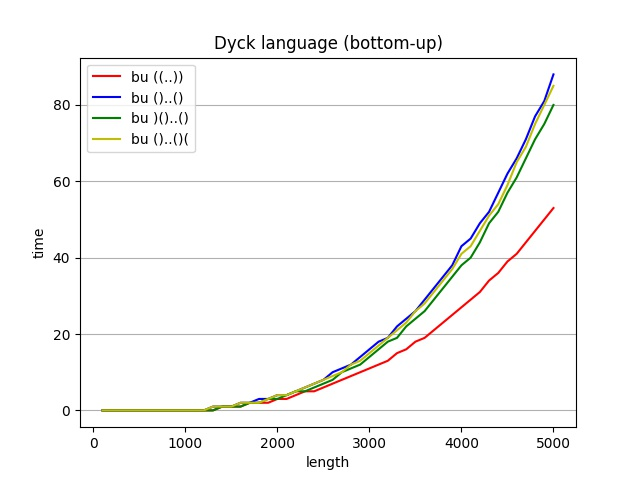
\includegraphics[width=0.6\textwidth]{Resources/t_dyck_bu.jpg}
    \caption{Running time (s) of the bottom-up algorithm when parsing different set of strings of sizes 100-5000, in steps of hundred, for the \textit{Dyck language}.}
    \label{fig:t_dyck_bu}
\end{figure}

Figure~\ref{fig:t_dyck_bu} shows the running times of the bottom-up parser on different sets of input strings for the grammar \textit{Dyck language}.
The strings were of length 100 to 5000, growing in steps of 100.
As expected, the times are very similar for three of the four different sets of input strings.
However, parsing the strings of the form \texttt{\texttt{((..))}}is a little faster.
When looking at how the $tab$ is filled, we see that $tab[A]$ is very similar in both cases.
$tab[S]$ on the other hand has \textit{true} in more cells for strings of the form \texttt{()..()} than \texttt{((..))}.
As we argued before, the loop over $k$ gets breaked, when both subproblems are true, which makes the parser more efficient.
Thus, more \textit{true} entries intuitively lead to faster running times, as the loop is executed less often.
For strings of the form \texttt{()..()}, this is not the case.
The additional \textit[true] in $tab[s]$ lead to a lot more table accesses, when the rule $S\rightarrow SS$ is considered.
Therefore strings of the form \texttt{\texttt{((..))}} can be parsed faster by the bottom-up algorithm.

The curves are asymptotically to $O(n^3)$, in fact, the yellow, blue and green line are very close to $6.4*10^{-10}*n^3$.

We split the parsings of top-down into two plots.
The first one, Figure~\ref{fig:t_dyck_td_slow}, is for the slow cases, where we did not run the parser on strings longer than 2500
The second one, Figure~\ref{fig:t_dyck_td_fast}, was for the fast cases, where we extended the test set to contain strings up to a size of 10000.

\begin{figure}[!ht]
    \centering
    \begin{subfigure}[b]{0.48\textwidth}
        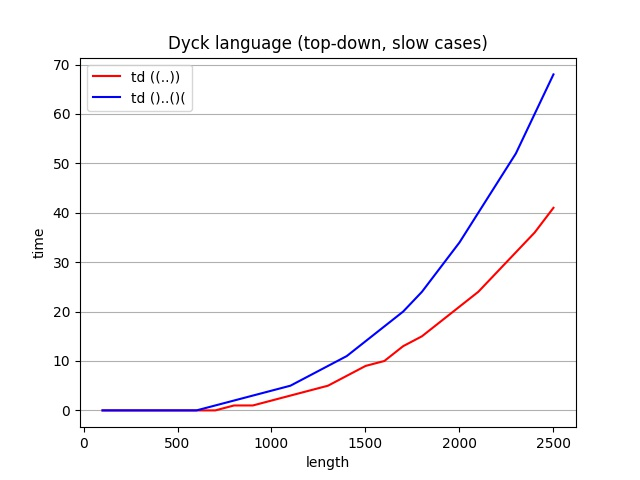
\includegraphics[width=1.1\textwidth]{Resources/t_dyck_td_slow.jpg}
        \caption{}
        \label{fig:t_dyck_td_slow}
    \end{subfigure}
    \hfill
    \begin{subfigure}[b]{0.48\textwidth}
        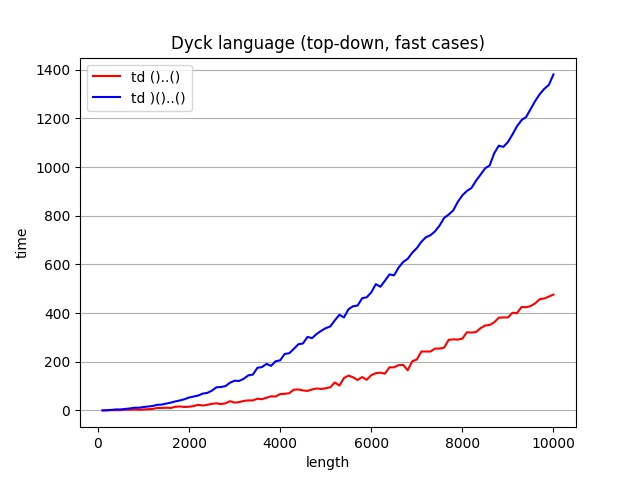
\includegraphics[width=1.1\textwidth]{Resources/t_dyck_td_fast.jpg}
    \caption{R}
    \label{fig:t_dyck_td_fast}
    \end{subfigure}
    \caption{Running times in (a) seconds and (b) milliseconds for the top-down algorithm when parsing four sets of strings of sizes (a) 100-2500 and (b) 100-1000, in steps of hundred, for the \textit{Dyck language}.}
\end{figure}

As we assumed, parsing the test sets of strings of the form \texttt{((..))}and \texttt{()..()(}with top-down was a lot slower than parsing the strings of the other two sets.
While parsing strings of the form \texttt{()..()(}of length 2500 took almost 70 seconds, parsing strings of the form \texttt{()..()}of length 10'000 took only 0.4 seconds.

The fast cases are a lot faster than the bottom-up parser.
This is the case, because bottom-up fills all cells of $tab$, regardless of whether or not they are needed to find the solution, while top-down only fills the one needed to find the optimal solution.
When the productions of the grammar are in a favorable order and the splitting points for finding subproblems that yield the optimal solution is low, as it is the case in the fast cases of Dyck, it can be very fast.

However, if this is not the case, then the parser may take a lot of time.
We can see this at the slow cases of the \textit{Dyck language}.
Here, the parser behaves a lot worse than bottom-up.
This may be due to the fact, that bottom-up fills the cells of $tab$ in a structured way, accessing the already filled cells of $tab$ not more often, then needed to fill the other cells.
Top-down on the other hand may run into the same subproblems very often.
This means the algorithm calls itself recursively in order to access the cell of the same subproblem more often than bottom-up does.
Since recursive calls are more time consuming, and more accesses may be performed, this results in a potentially very bad running time.

\begin{figure}[!ht]
    \centering
    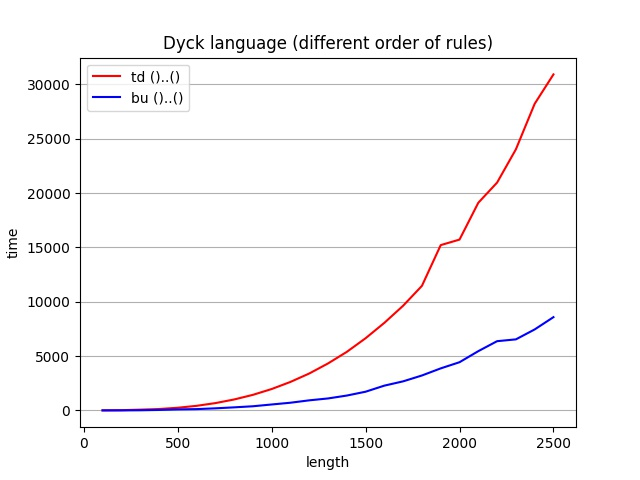
\includegraphics[width=0.6\textwidth]{Resources/t_dyck_order.jpg}
    \caption{Running time (ms) of both algorithms for parsing a set of strings of sizes 100-2500, in steps of hundred, for the \textit{Dyck language}, with a different order of the productions.}
    \label{fig:t_dyck_order}
\end{figure}

I order to verify the hypothesis, that the order of productions matters for the top-down parser, we run experiments on the same grammar, but with the productions of $S$ in opposite order.
The results can be seen in figure~\ref{fig:t_dyck_order}.
The parser is in fact a lot slower than it was before, thus the order of the productions may play a major role, when parsing.
The plot further shows that the order does not matter that much for the bottom-up parser.
It has almost the same running time, than it had with the original ordering of the productions.

\subsubsection{Strings starting and ending in a}

As expected, both the top-down and bottom-up algorithm performed very differently on the two grammars, being rather fast at parsing for the grammar \textit{starting in a}, and slower for \textit{ending in a}.
In general, we see that the times are lower than they were for the \textit{Dyck language}.
This is presumably because this grammar has only two non-terminal productions, which leads to less subproblems which have to be considered.

We split the results in three graphs; one for the running times of both parsers on the grammar \textit{ending in a} (Figure~\ref{fig:t_ea_td_bu}), one for top-down and one for bottom-up, each for the grammar \textit{starting in a} (Figures~\ref{fig:t_sa_td} and~\ref{fig:t_sa_bu} respectively).

\begin{figure}[!ht]
    \centering
    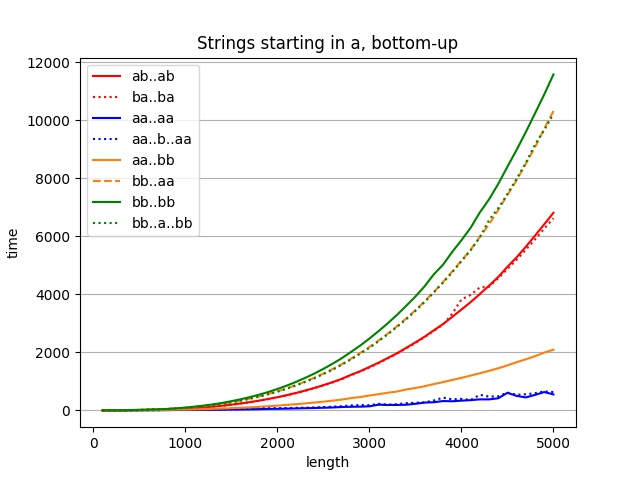
\includegraphics[width=0.6\textwidth]{Resources/t_sa_bu.jpg}
    \caption{Running time (ms) of the bottom-up algorithm when parsing sets of strings of sizes 100-2500, in steps of hundred, for the language of words starting in a.}
    \label{fig:t_sa_bu}
\end{figure}

Figure~\ref{fig:t_sa_bu} shows, that the running times of bottom-up indeed depends on the amount of \texttt{b}'s in the input string.
We see, that strings of the form \texttt{bb..bb} have the slowest running times, while strings of the form \texttt{aa..aa} are parsed very fast.
While adding an \texttt{a} to the first type does influence the running time, adding a single \texttt{b} to the second one has almost no influence.
Further, for strings with alternating letters (the red lines) the running time does not change if the string starts with \texttt{a} or \texttt{b}.
However, if the \texttt{a}'s and \texttt{b}'s are continuously (yellow lines), the strings are parsed a lot faster if the \texttt{a}'s are first.
\todo{add further analysy/reasoning?}

\begin{figure}[!ht]
    \centering
    \begin{subfigure}[b]{0.48\textwidth}
        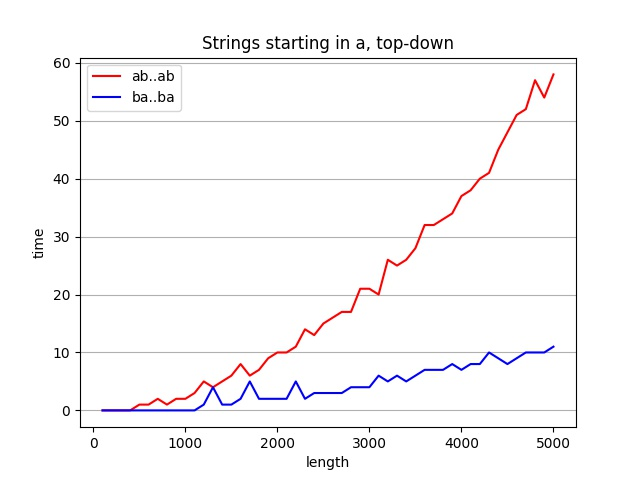
\includegraphics[width=1.1\textwidth]{Resources/t_sa_td.jpg}
        \caption{}
        \label{fig:t_sa_td}
    \end{subfigure}
    \hfill
    \begin{subfigure}[b]{0.48\textwidth}
        \centering
        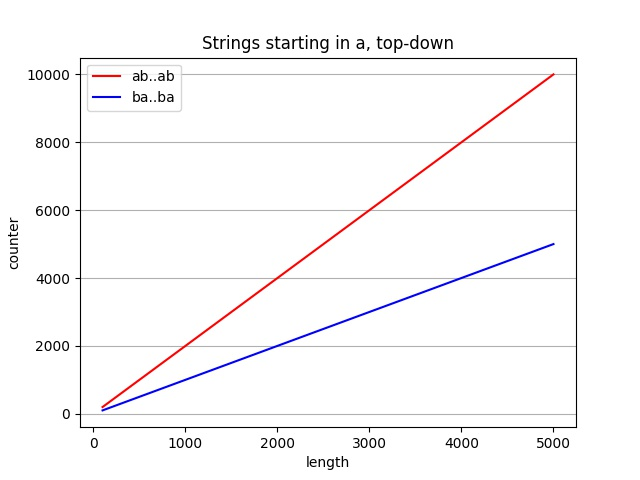
\includegraphics[width=1.1\textwidth]{Resources/c_sa_td.jpg}
        \caption{}
        \label{fig:c_sa_td}
    \end{subfigure}
    \caption{Sunning time in ms (a) and counter (b) of the top-down algorithm when parsing sets of strings of sizes 100-5000, in steps of hundred, for the Language of words starting in a.}
\end{figure}

Figure~\ref{fig:t_sa_td} shows the incredibly low running times of top-down on the grammar \textit{strings starting in a}.
The times are so low, since the algorithm does not fill $tab$ completely.
In fact, when parsing strings not starting in \texttt{a}for the grammar \textit{starting in a}, it will only ever look at the most left children of the recursive tree, since each of them returns \textit{false}.
This results in a very low amount of recursive calls as can be seen in figure~\ref{fig:c_sa_td}.
The number of calls on the recursive function is $\Theta(n)$ for parsing strings not starting in a for the grammar \textit{starting in a}.
As we argued in section~\ref{sec:top_down}, the upper bound for this number is $O(n^3)$.
The numbers for the counter of bottom-up (repetitions of the inner most loop, i.e. over splitting points $k$) for parsing strings for \textit{starting in a}, are somewhere in between of $n^2$ and $n^3$, still yielding relatively fast running times.

The three bumps in the running time of top-down on strings of the form \texttt{ba..ba}are supposedly due to rounding errors of the compiler, seen as the times there are lower than 5 milliseconds.
The bumps appear on the red line at the same time after the same period of time after starting the parsers (not at the same length of strings!), though not as distinctive as in the blue line, since the running times are already a little higher at this point.
The bumps could be reduced by running the parser 40 times per input string instead of 10 times which supports this theory.

\begin{figure}[!ht]
    \centering
    \begin{subfigure}[b]{0.48\textwidth}
        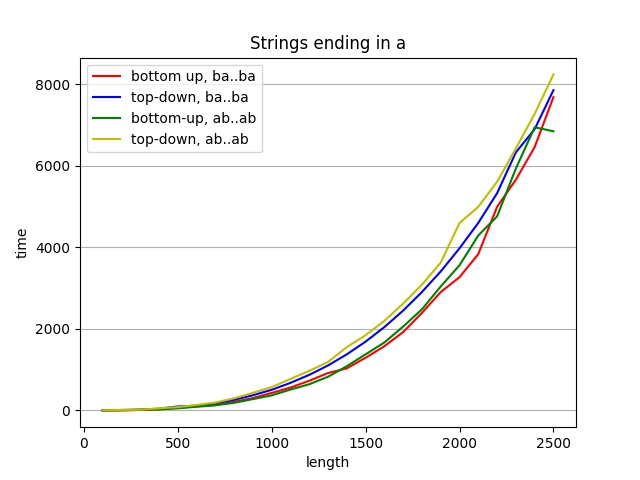
\includegraphics[width=1.1\textwidth]{Resources/t_ea_td_bu.jpg}
        \caption{}
        \label{fig:t_ea_td_bu}
    \end{subfigure}
    \hfill
    \begin{subfigure}[b]{0.48\textwidth}
        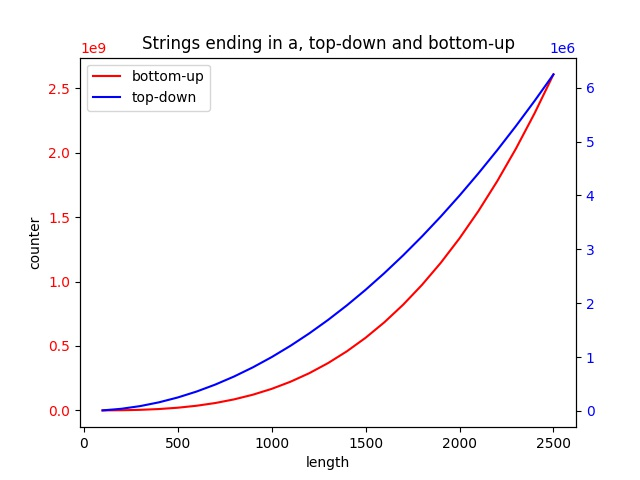
\includegraphics[width=1.1\textwidth]{Resources/c_ea_td_bu.jpg}
        \caption{}
        \label{fig:c_ea_td_bu}
    \end{subfigure}
    \caption{Running time in ms (a) and counter (b) of the bottom-up and top-down algorithm when parsing sets of strings of sizes 100-2500, in steps of hundred, for the language of words ending in a.}
\end{figure}

Figures~\ref{fig:t_ea_td_bu} and \ref{fig:c_ea_td_bu} show, that the curves for parsing the grammar \textit{ending in a} are almost identical with the ones of the bottom-up parser run on the \textit{Dyck language}.
We further see, that all of them have a very similar shape.
In fact, both the bottom-up and the top-down parser have the same counter respectively for any string of the same length, regardless of the order of the letters.
As can be seen in figure\ref{fig:c_ea_td_bu}, for a string of length 100, bottom-up iterates 171600 times of its most inner loop while top-down calls itself recursively 9901 times.
Despite this big difference of \texttt{counter}, the running times are almost identical for both algorithms.
This is due to the more efficient manner of bottom-up.
One aspect is the more structured way to allocate the cells of $tab$, the second one the fact that Java can not perform recursive functions as efficient as iterative ones. \todo{is here a citation needed?}


\subsection{Evaluation of the Specialization with Linear Grammars}
In order to test the specialization for linear grammars, we parse strings by using the grammar parser, which transforms the linear grammar provided to CNF.
Further, we compare the running times of parsing strings with the transformed grammar to parsing them with the specialized bottom-up algorithm.

\subsubsection{Grammar Transformation}
In order to test how parsing the grammar from a linear grammar to on in CNF, we use the linear form of the \textit{Dyck language} as introduced in \ref{par:dyck_linear}.
The comparison of those results to the results fo the evaluation of the initial \textit{Dyck Language} can be seen in figure~\ref{fig:t_c_dyck_lin_cnf}.
As expected, strings could be parsed slightly faster for the transformed grammar than for the initial form.
The plot further shows, that the linear bottom-up algorithm is a lot faster than the CNF one, and that the counter is perfectly asymptotical to the running time.

\begin{figure}[!ht]
    \centering
    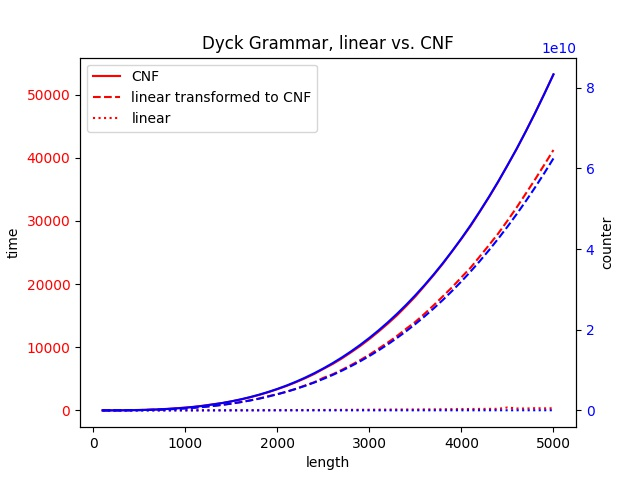
\includegraphics[width=0.6\textwidth]{Resources/t_c_dyck_lin_cnf.jpg}
    \caption{Running time (ms) and counter of the bottom-up algorithm when parsing strings of the form \texttt{((..))} for the Dyck language. \textit{CNF} is the running time of parsing with the productions of the initial grammar, \textit{linear transformed to cnf} the one for the linear productions, but transformed to CNF by the parser, and \textit{linear} the running times when the specialized CYK algorithm was used.}
    \label{fig:t_c_dyck_lin_cnf}
\end{figure}

The CNF-configuration refers to the bottom-up parser run on the initial grammar, time and counter are the same as in \ref{sec:eval_dyck}.
The second configuration used the linear transformation of the \textit{Dyck language}, but transformed it to CNF before parsing the strings.
This results in one non-terminal rule less, which is why the parser is slightly faster.
The third configuration parses strings for the linear grammar using the specialized algorithm.
It is a lot faster then both of the other configurations.
To analyse the difference between the linear and CNF parser better, we consult the experiments run on the \textit{abc grammar}.


\subsubsection{Adapted algorithm}
\begin{figure}[!ht]
    \centering
    \begin{subfigure}[b]{0.48\textwidth}
        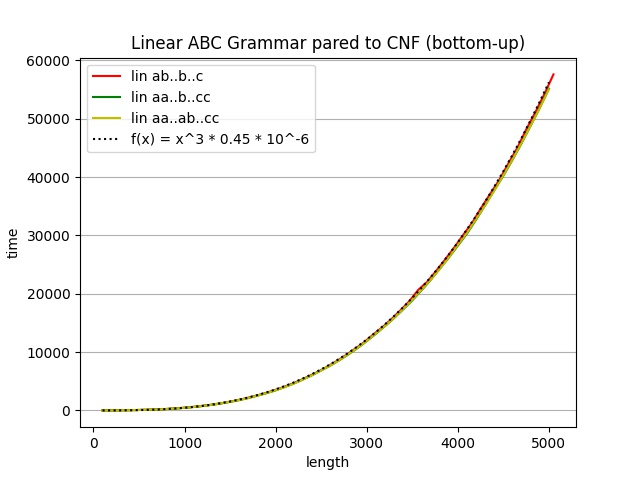
\includegraphics[width=1.1\textwidth]{Resources/t_abc_cnf.jpg}
        \caption{}
        \label{fig:t_abc_cnf}
    \end{subfigure}
    \hfill
    \begin{subfigure}[b]{0.48\textwidth}
        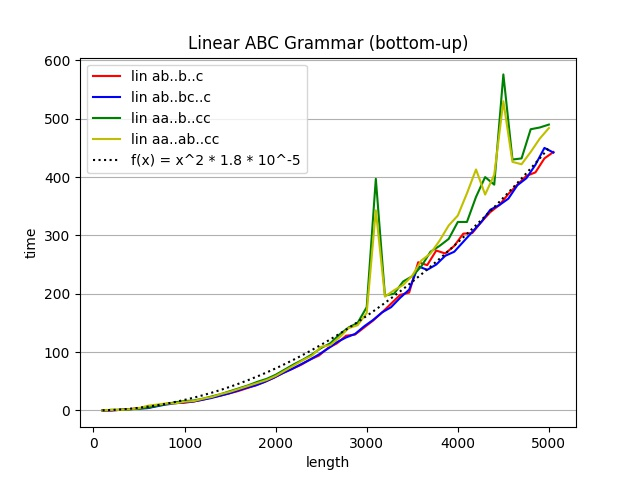
\includegraphics[width=1.1\textwidth]{Resources/t_abc_lin.jpg}
        \caption{}
        \label{fig:t_abc_lin}
    \end{subfigure}
    \caption{Running time in ms of the bottom-up algorithm when parsing strings for a linear grammar (a) by transforming the grammar to CNF and (b) by using the specialized algorithm. Both plots contain a function of the length as reference.}
\end{figure}

Figure \ref{fig:t_abc_cnf} shows the running time which is yielded when parsing strings for the \textit{abc grammar} by transforming the productions to CNF.
Since we used the bottom-up parser we expected the times to be very similar for all sets of input strings, which is the case.
The graph also contains a function over the length of the input strings, $f(x)=x^3*0.45*10^-6$, which shows that the running time indeed is in $O(n^3)$.
The specialized algorithm could parse the strings in a tenth of the time, the cnf parser needed.
This is partly due to the smaller amount of rules, but also because only one splitting point per rule has to be considered.
Here, the running times are very similar for all types of input strings, too.
The variations between the different types can be seen better, as the numbers are a lot smaller.
Like in Figure~\ref{fig:t_dyck_td_fast}, some configurations have bumps.
We explain them with the same reasoning, assuming they appear only because the algorithm is very fast.
The graph, too, contains a function over the length of the input strings, $f(x)=x^2*1.8*10^-5$,showing that the running time is in $O(n^2)$, as expected.

\section{Conclusion}

\todo{summarize the outcome of the experiments and draw some further conclusions.}

Bottom-up is very steady, it's behavior can easily be predicted, as it is mainly dependent on the length of the input string.
Top-down on the other hand, since it only looks at subproblems that are needed to find the optimal solution, can be a lot faster.
When the rules of the grammar are in the correct order, i.e., in an order such that the rules used for optimal solutions are considered first, and the splitting points to find said solutions are low, then this parser will yield very good running times.
If neither is the case, it can be a lot slower than bottom-up, since bottom-up fills the cells in a structured way and thus accesses the cells less often.
Top down may access the same cell a lot of times, when the same subproblem occurs very often, resulting in a bad.

\todo{Bibliography. Cited works are mainly both books used in the lecture.}



\pagebreak
\printbibliography

\end{document}
